%% Corrects the page numbering, there is no need to change these
\cleardoublepage
\setcounter{page}{1}
\pagenumbering{arabic}

%% Leave first page empty \thispagestyle{empty}
\chapter{Introduction} 
The relationship between human beings and space has existed since the beginning of time. It has always been a source of mystery, something we want to understand. More than 4000 years ago, the Egyptians and the Babylonians were influenced by the movements of the sun and the planets and, based on those movements, developed calendars for their crops. Later, the ancient Greeks developed the concept of \emph{astronomy}, the science of the heavens. Subsequently, we can find philosophers such as Nicolaus Copernicus, Johannes Kepler, who explained the motion of the planets, and Galileo Galilei. In the 17th century, Sir Isaac Newton invented calculus, developed his law of gravitaion and performed important experiments in optics.\\

The technological advancements of the 20th century, specially accelerated by the World War II, made physical exploration of space become possible. This thesis is oriented towards one of those advancements, artificial satellites.\\

A \emph{satellite} is a natural or artificial object moving around a bigger body. This motion is defined as an orbit, enabled by the dominant force of gravity from the bigger body. In early 1945, the United States started the Vanguard Rocket development to launch a satellite. However, after several failed launches, it was de Soviet Union who took the advantage by launching the Sputnik-1 (Figure \ref{f1.1}) on October 4, 1957. During the Cold War, the space race between the Sovient Union and the United States was a hard fight which made space technology advance quite rapidly.\\

\begin{figure}[H]
\centerline{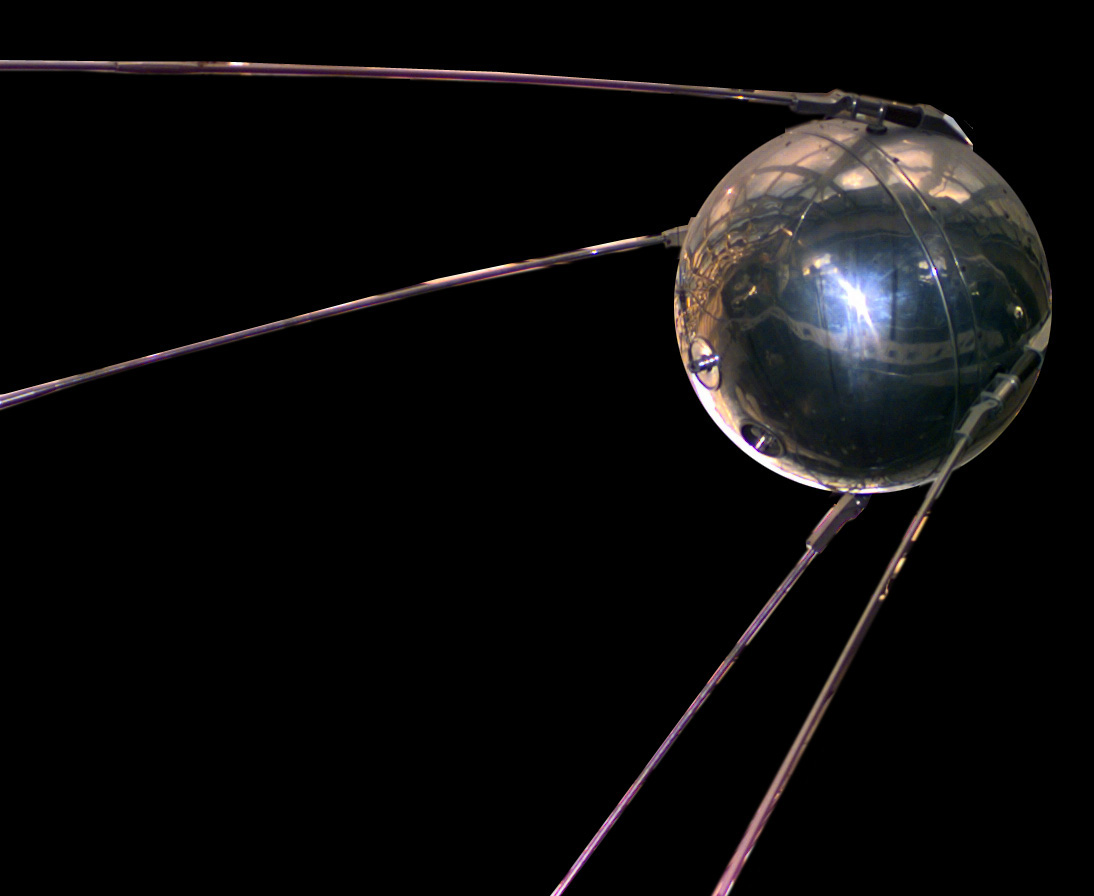
\includegraphics[width=0.7\textwidth]{images/sputnik.jpg}}
\caption{Sputnik 1 (NASA Public Domain)}
\label{f1.1}
\end{figure}

Finally, on January 31, 1958 the United States managed to launch their first artificial satellite, the Explorer-1 (Figure \ref{f1.2}).\\
\begin{figure}[H]
\centerline{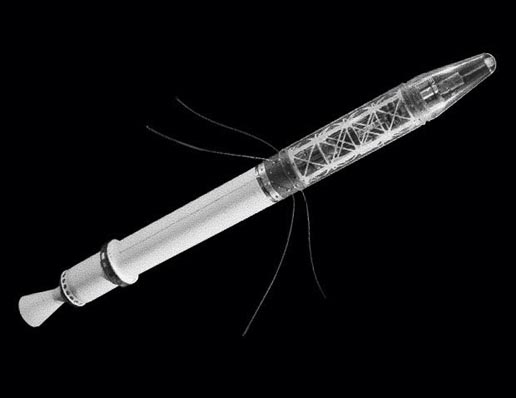
\includegraphics[width=0.7\textwidth]{images/explorer1.jpg}}
\caption{Explorer 1 (NASA Public Domain)}
\label{f1.2}
\end{figure}
\pagebreak

As of October 1, 2011 there were 966 operating satellites in orbit. About two-thirds of these were owned by the United States, Russia and China\cite{SBFE}. Their major types are:
\begin{itemize}
\item Communications: used for television, radio, Internet and telephone services.
\item Navigation: using radio time signals, this satellites allow mobile receivers on the ground to determine their exact position. They are also used to determine the location of satellites situated in lower orbits.
\item Exploration: used to observe distant planets, galaxies and other outer space objects by using telescopes and other sensors.
\item Remote sensing: Remote sensing satellites are used to gather information about the nature and condition of Earth. The sensors in this kind of satellites receive electromagnetic emissions in several spectral bands and can detect the object's composition and temperature. Also, environmental conditions and so on. These satellites have also been widely used as military "spy satellites".

\end{itemize}

The constant evolution of technology and the growth of human needs have me the mission requirements rise throughout the last decades, thus, satellite mass has grown from Sputnik's 84 kg. and Explorer-1's 14k kg. to over 6,000 kg in 2007\cite{BARN}. The main consequence of this, amongst others, has been an increment in mission costs.\\

To counter this trend, the small satellite movement was created by the academic community and it has shown how mission costs can be cut dramatically to a point in which a university can build a launch their own satellite. (Figure \ref{f1.3}). Due to its success, it has become vigorous industry. Aalto-1 and ESTCube-1, projects with which this thesis is related, are nanosatellites, and the perfect example of this new concept.\\

\begin{figure}[H]
\centerline{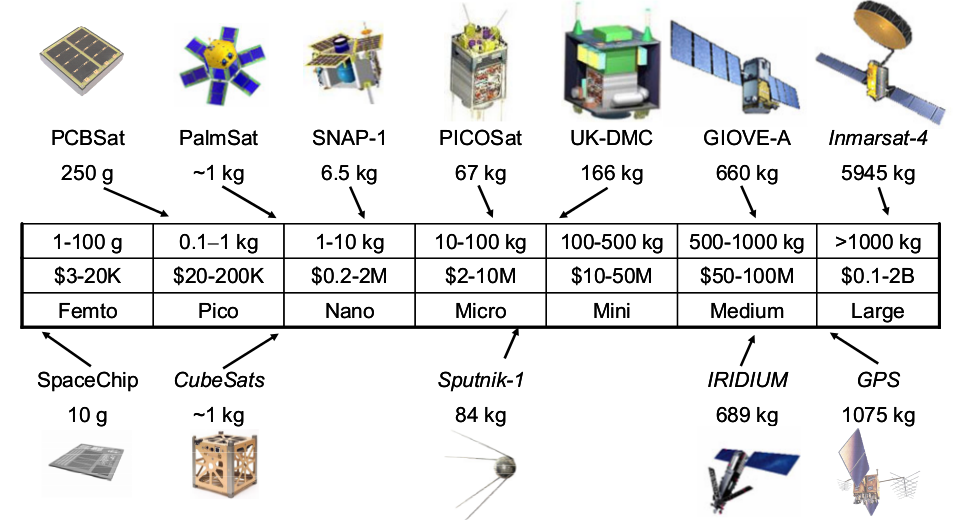
\includegraphics[width=0.7\textwidth]{images/satclass.png}}
\caption{Satellite Mass and Cost Classification \cite{BARN}}
\label{f1.3}
\end{figure}

\section{Background}\label{1.1}

As it was stated before, this thesis is closely related to two different projects. Aalto-1 and ESTCube-1. These two projects are based on the most common standard use by universities, CubeSat\cite{CubeSat}. An open standard developed by the California Polytechnic State University and Stanford University.

\subsection{Aalto-1}

Led by Aalto University, Aalto-1 project aims to build a multi-payload remote sensing nanosatellite (Figure \ref{f1.4}). The size of the satellite is approximately 34 cm x 10 cm x 10 cm with a mass of less than 4 kg\cite{AALTO1a}. Aalto-1 will also be the first Finnish satellite.

\begin{figure}[H]
\centerline{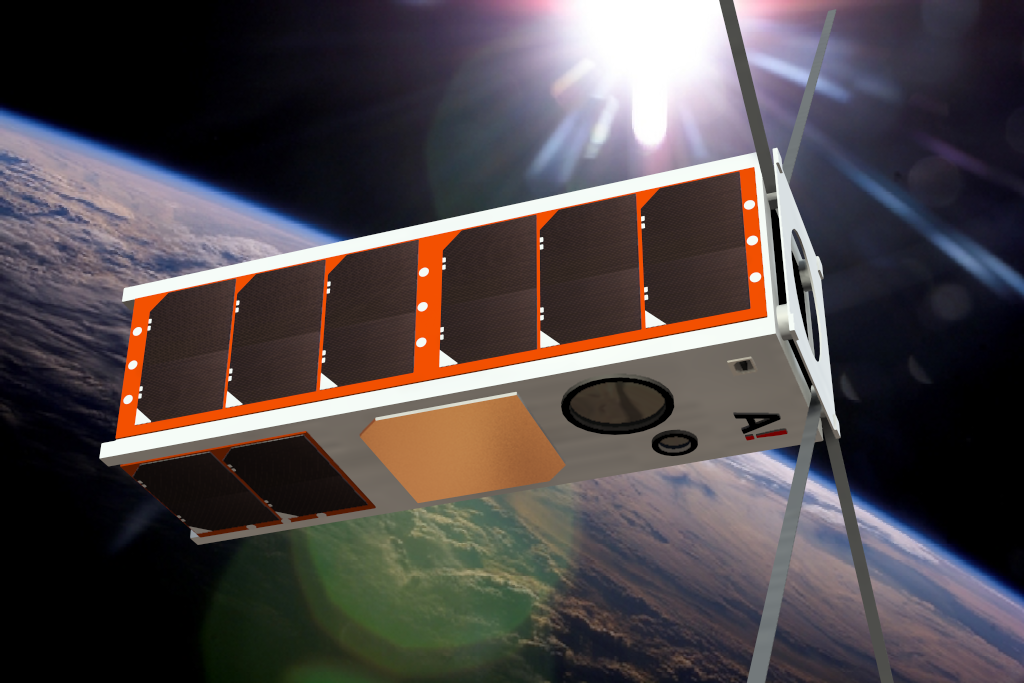
\includegraphics[width=0.7\textwidth]{images/aalto1.png}}
\caption{Aalto-1}
\label{f1.4}
\end{figure}


There are different institutions cooperating to make this possible. The main payload, the imaging spectrometer, has been designed and built by VTT Technical Research Centre of Finland. The Radiation Monitor (RADMON) has been designed by the Universities of Helsinki and Turku in cooperation with the Finnish Meteorological Institute (FMI). The Plasma Brake has been designed by a consortium including the FMI, the Department of Physics of the University of Helsinki, the Departments of Physics and Astronomy and Information Technology of the University of Turku, the Accelerator laboratory of the University of Jyväskylä, Aboa Space Resarch Oy, Oxford Instruments Oy and other Finnish companies. Meanwhile, Aalto University is responsible for designing and building the satellite platform and the day-to-day operation of the project.\cite{AALTO1b}\\
\newpage
Aalto-1's mission is to validate the technologies used by the payloads in space environment and measure their performance. In addition, it is also an educational project. Students are the main workforce towards its success. Being the the first Finnish student satellite mission, is a good tool to improve Finnish space teaching and also allow students to be in touch with prominent partners, both domestic and international, in the space technology field.


\subsection{ESTCube-1}

ESTCube-1 is a single-unit CubeSat (Figure \ref{f1.5}). The size of the satellite is approximately 10 cm x 10 cm x 10 cm with a maximum mass of 1.33 kg. It has been build by students of the universities of Tartu and Tallinn, in Estonia, and it is the first Estonian satellite \cite{ESTCube}.
It was launched from the Guaiana Space Centre on May 7, 2013 as one of the three payloads of the Vega VV02 rocket \cite{Arianespace}.\\

\begin{figure}[H]
\centerline{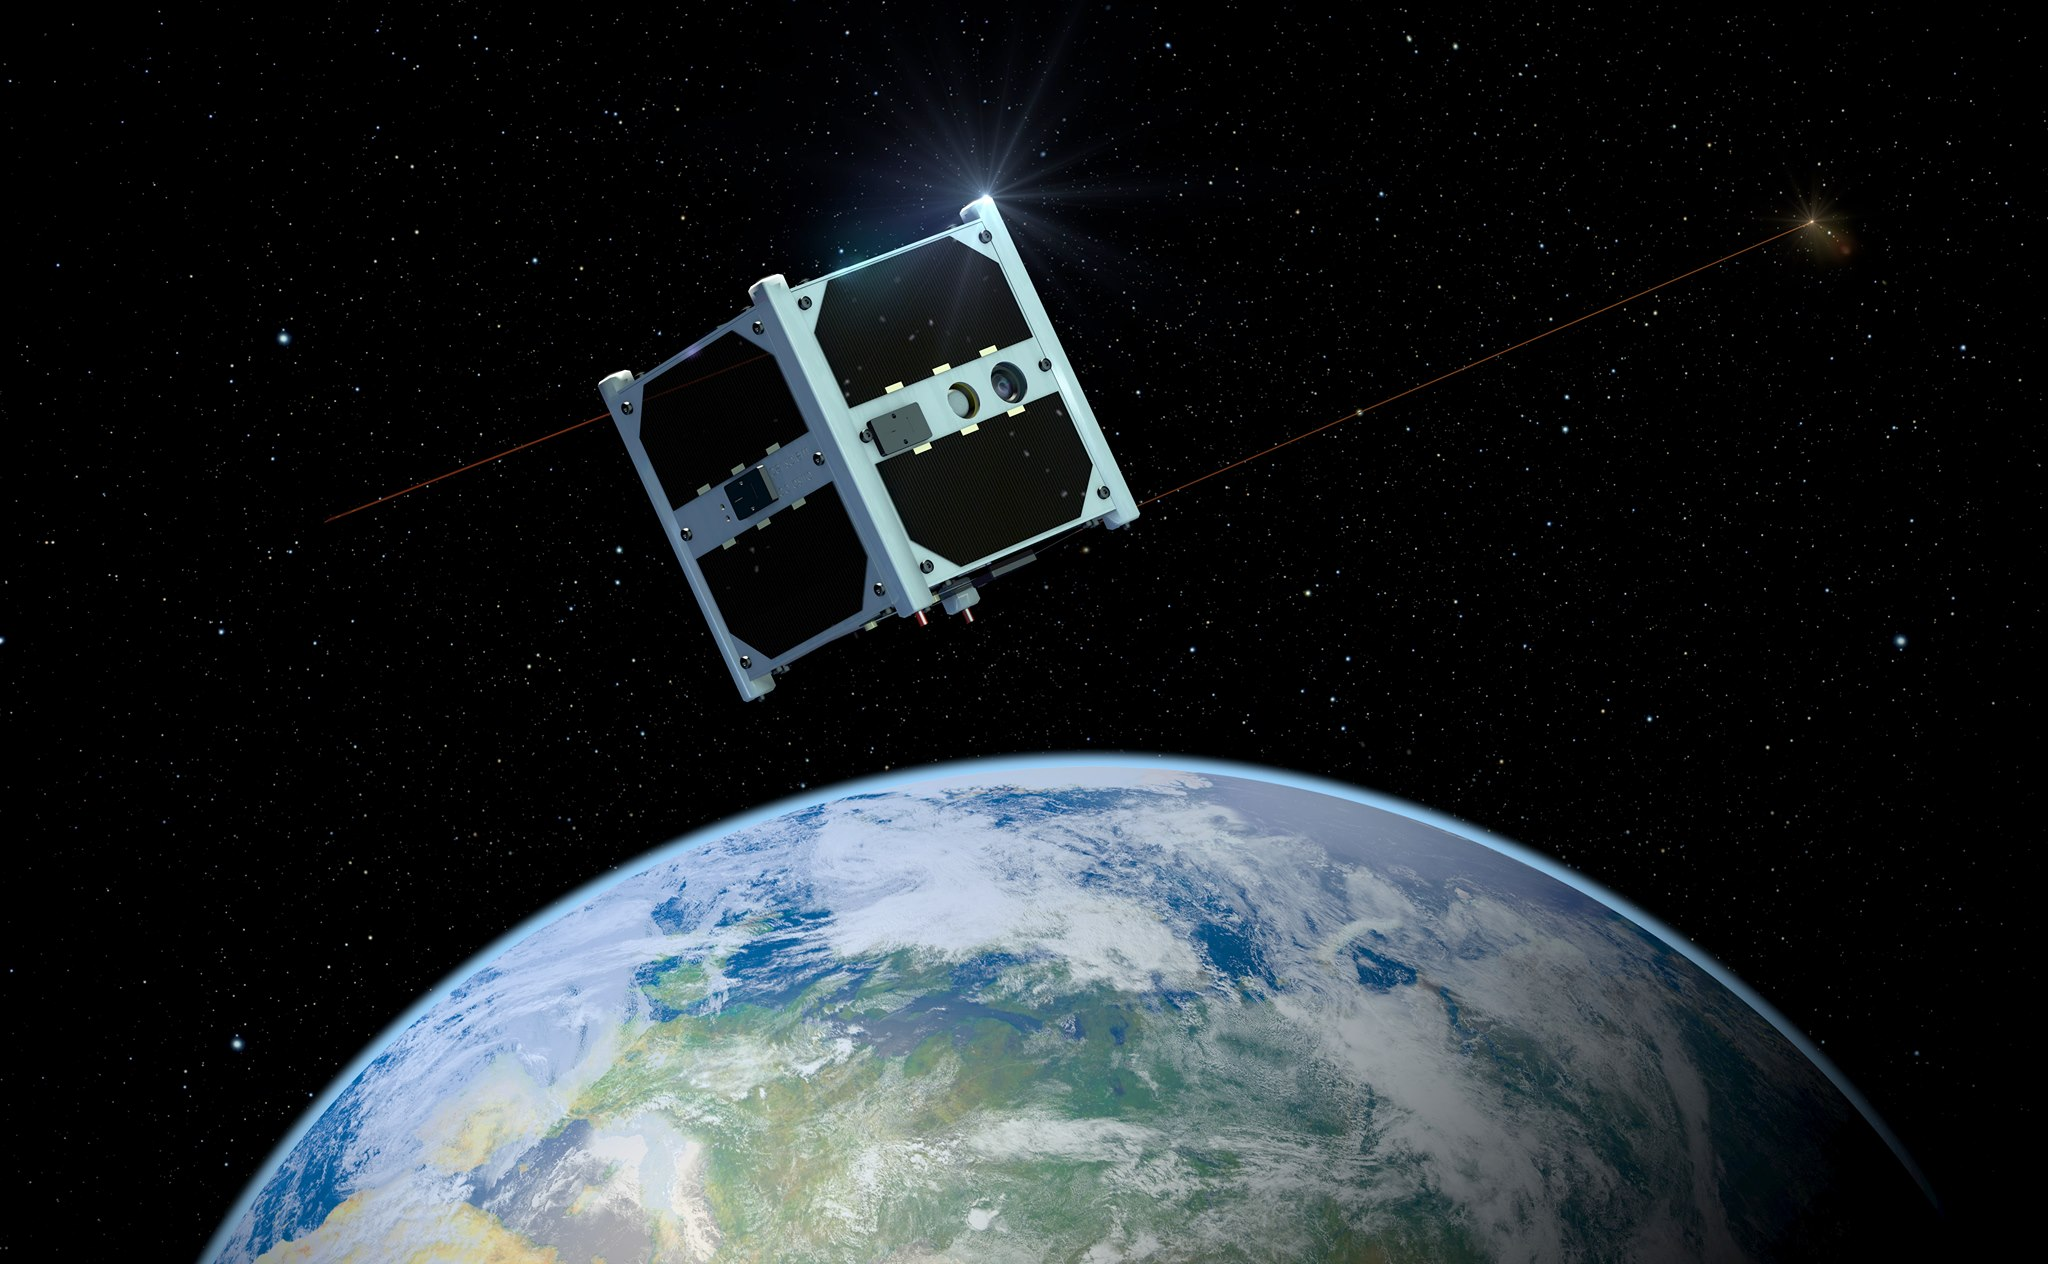
\includegraphics[width=0.7\textwidth]{images/ESTCube.jpg}}
\caption{ESTCube-1}
\label{f1.5}
\end{figure}

ESTCube-1's main goal is to observe and measure the E-sail effect for the first time. It has been placed into a polar low Earth orbit (LEO) and will deploy a single 10 m long and 9 mm wide tether\cite{ESTCube}. This has relation with Aalto-1's Plasma Brake, which will deploy a 100 m long tether. The require duration of ESTCube-1's mission is a few weeks and it can be extended to about a year.



\section{Problem statement}\label{1.2}


\section{Research objectives and scope}

The purpose of this thesis is to develop a calibration system for a ground station which will solve the problem mentioned above. In addition, it is necessary to check if the received values are within a expected range, so a different system will be developed for that purpose.\\

Using ESTCube-1 project as a baseline, the author aims to develop such systems which are generic enough to be used by any number of satellite missions. The modules developed will be integrated into \emph{Hummingbird}, an open source platform for monitoring and control which will be explained later in this work. 





\section{Motivations}



\section{Outline of the thesis}


\newpage
